%!TEX TS-program = pdflatex
%!TEX encoding = UTF-8 Unicode
% -*- coding: utf-8 -*-

\documentclass[10pt]{beamer}
%\usepackage[english]{babel} 
%\usepackage[dvipdfmx]{movie15_dvipdfmx}
\usepackage{color}
\usepackage{tikz}
\usetikzlibrary{calc,arrows,shapes.multipart}
\usepackage{multicol}

\usepackage{listings}
%\usepackage{algpseudocode}
%\usepackage{algorithmic}
\definecolor{solarized@base03}{HTML}{002B36}
\definecolor{solarized@base02}{HTML}{073642}
\definecolor{solarized@base01}{HTML}{586e75}
\definecolor{solarized@base00}{HTML}{657b83}
\definecolor{solarized@base0}{HTML}{839496}
\definecolor{solarized@base1}{HTML}{93a1a1}
\definecolor{solarized@base2}{HTML}{EEE8D5}
\definecolor{solarized@base3}{HTML}{FDF6E3}
\definecolor{solarized@yellow}{HTML}{B58900}
\definecolor{solarized@orange}{HTML}{CB4B16}
\definecolor{solarized@red}{HTML}{DC322F}
\definecolor{solarized@magenta}{HTML}{D33682}
\definecolor{solarized@violet}{HTML}{6C71C4}
\definecolor{solarized@blue}{HTML}{268BD2}
\definecolor{solarized@cyan}{HTML}{2AA198}
\definecolor{solarized@green}{HTML}{859900}
\lstset {
  language=python,
%  upquote=true,
%  columns=fixed,      tabsize=4,
%  extendedchars=true, breaklines=true,
%  frame=tb,
%  rulesepcolor=\color{solarized@base03},
%  numberstyle=\tiny\color{solarized@base01},
  basicstyle=\scriptsize\ttfamily,
  keywordstyle=\color{solarized@green},
  stringstyle=\color{solarized@cyan}\ttfamily,
  identifierstyle=\color{solarized@blue},
  commentstyle=\color{solarized@base01},
  emphstyle=\color{solarized@red}
}
 

\definecolor{blendedblue}{rgb}{0.2, 0.2, 0.7} 

%% % --- Font --------------------------------------------------------------------
%% \usepackage{fontspec} 
%% \fontspec[Weight=1.0,Scale=1.0]{Gill Sans Light}
%% \setsansfont [
%%   Mapping = tex-text,
%%   Ligatures={Common},
%%   Numbers=OldStyle,
%%   Scale=.9,
%%   BoldFont={Gill Sans},
%%   ItalicFont={Gill Sans Light Italic}
%% ]{Gill Sans Light}
%% \setmainfont [
%%   Mapping = tex-text,
%%   Ligatures={Common},
%%   Numbers=OldStyle,
%%   BoldFont={Gill Sans},
%%   ItalicFont={Gill Sans Light Italic}
%% ]{Gill Sans Light}

% --- Beamer theme ------------------------------------------------------------
\usetheme{Pittsburgh}
%\useoutertheme[footline=empty,subsection=false]{miniframes}
%% \useoutertheme[subsection=false]{miniframes}
\setbeamertemplate{navigation symbols}{} %no nav symbols
%% \setbeamercolor{section in head/foot}{use=normal text,bg=white}
%% \setbeamertemplate{section in head/foot shaded}[default][25]
%% \setbeamerfont{title}{family={\fontspec[Weight=0.5,Scale=1.25]{Gill Sans}}}
%% \setbeamerfont{subtitle}{family={\fontspec[Weight=0.5,Scale=1]{Gill Sans Light}}}
%% \setbeamerfont{frametitle}{family={\fontspec[Weight=1.0,Scale=1.1]{Gill Sans}}}
%% \setbeamerfont{framesubtitle}{family={\fontspec[Weight=0.5,Scale=1.]{Gill Sans Light}}}



% Docmument title, author, date and institution
% ---------------------------------------------
\title{Vispy\\
{\small A Modern and Interactive Visualization Framework}}
\author{Luke Campagnola, Almar Klein, Cyrille Rossant\\ \& {\bf Nicolas Rougier} (it's me)} 
\date{EuroSciPy 2013\\

\includegraphics[width=0.15\textwidth]{vispy-logo}}

\begin{document}

\begin{frame}
  \titlepage
\end{frame}

% -----------------------------------------------------------------------------
\begin{frame}
  \frametitle{}
  \begin{block}{}
    \begin{center}
      Our goal is to create a {\bf interactive} visualization\\ software in
      Python based on OpenGL/WebGL.\\
      \vspace{2.5mm}
      \includegraphics[height=4cm]{vispy}\\
      \vspace{2.5mm}
      We do not aim at replacing matplotlib.\\
      We aim at living by its side.\\
    \end{center}
  \end{block}
\end{frame}


% -----------------------------------------------------------------------------
\begin{frame}
  \frametitle{Python/OpenGL frameworks}

  \begin{block}{Rendering framework}
    \begin{multicols}{2}
      \begin{itemize}
      \item Pyglet\\
        {\scriptsize \url{www.pyglet.org}}
      \item PyOpenGL\\
        {\scriptsize \url{pyopengl.sourceforge.net}}
      \item Nodebox for OpenGL\\
        {\scriptsize \url{www.cityinabottle.org/nodebox}}
      \item PyProcessing\\
        {\scriptsize \url{code.google.com/p/pyprocessing}}
      \end{itemize}
    \end{multicols}
  \end{block}

  \begin{block}{Visualization framework}
    \begin{multicols}{2}
    \begin{itemize}
    \item mayavi 2 {\scriptsize (Enthought)}\\
      {\scriptsize \url{github.com/enthought/mayavi}}
    \item VTK {\scriptsize (Kitware)}\\
      {\scriptsize \url{www.vtk.org}}
    \item \textcolor{red}{galry {\scriptsize (Cyrille Rossant)}}\\
      {\scriptsize \url{rossant.github.io/galry/}}
    \item \textcolor{red}{visvis {\scriptsize (Almar Klein)}}\\
      {\scriptsize \url{code.google.com/p/visvis/}}
    \item \textcolor{red}{glumpy {\scriptsize (Nicolas Rougier)}}\\
      {\scriptsize \url{code.google.com/p/glumpy/}}
    \item \textcolor{red}{pyqtgraph {\scriptsize (Luke Campagnola)}}
      {\scriptsize \url{www.pyqtgraph.org}}
    \end{itemize}
    \end{multicols}
  \end{block}

  %% \begin{columns}
  %%   \begin{column}{.45\textwidth}
  %%     \begin{block}{}
  %%     \end{block}
  %%   \end{column}
  %%   \begin{column}{.45\textwidth}
  %%   \end{column}
  %% \end{columns}

  %%   \begin{itemize}
  %%   \item mayavi
  %%   \item pyglet
  %%   \item processings / pyprocessings
  %%   \item nodebox / nodebox OpenGL
  %%   \item glumpy
  %%   \item galry
  %%   \item visvis
  %%   \end{itemize}
  %% \end{block}
\end{frame}


% -----------------------------------------------------------------------------
\begin{frame}
  \frametitle{Graphic cards}
  \framesubtitle{video-gaming industry is working for us !}

  \begin{center}
    \includegraphics[width=.75\textwidth]{cpu-vs-gpu.png}
  \end{center}
\end{frame}

% -----------------------------------------------------------------------------
\begin{frame}
  \frametitle{OpenGL history}
  \framesubtitle{}
  \input{opengl.tikz}
  \vfill
  \includegraphics[height=2cm]{doom.jpg}
  \hfill
  \includegraphics[height=2cm]{rage.jpg}\\
  \small Doom (1993) \hfill Rage (2011)
%  \vfill
%  2001: Final FantasyMovie, 90 minutes per frame using 900 CPUs\\
%  2013: 1 GPU, 1 CPU, real time
\end{frame}


% -----------------------------------------------------------------------------
\begin{frame}
  \frametitle{OpenGL ES 2.0 pipeline overview}
  \framesubtitle{(\url{openglinsights.com})}

  Around 350 constants and 150 functions.
  \begin{center}
    \includegraphics[width=1.0\textwidth]{GLES-Pipeline-2.png}
  \end{center}
\end{frame}

% -----------------------------------------------------------------------------
\begin{frame}
  \frametitle{OpenGL 4.2 pipeline overview}
  \framesubtitle{(could have been worse...)}

  Around 2000 constants and 1000 functions.
  \begin{center}
    \includegraphics[width=0.75\textwidth]{GL-Pipeline-4.png}
  \end{center}
\end{frame}


% -----------------------------------------------------------------------------
\begin{frame}
  \frametitle{Vispy pipeline overview}
  \framesubtitle{Data centered}
%  \begin{block}{}
    \begin{center}
      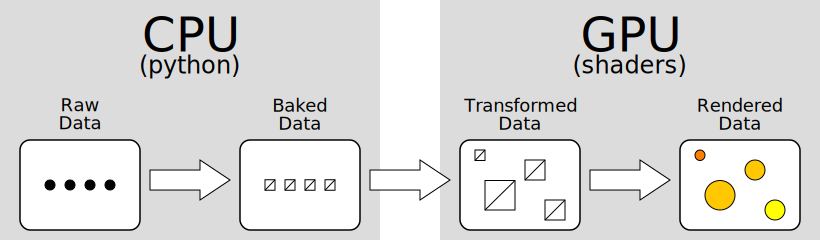
\includegraphics[width=1.0\textwidth]{vispy-pipeline}
    \end{center}
%  \end{block}
    Critical parts are the {\bf baking} process and the {\bf transfer} to GPU memory.\\
%    (using geometry shaders, we could deport (some) baking on the GPU).
\end{frame}

% -----------------------------------------------------------------------------
\begin{frame}
  \frametitle{Baking process}
  \begin{block}{Ideal case: no baking}
    \begin{columns}
      \begin{column}{.50\textwidth}
        \begin{center}
          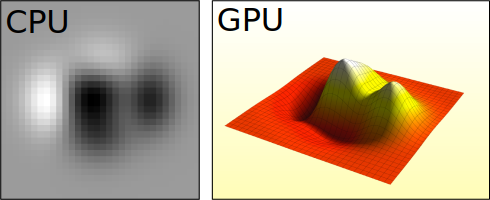
\includegraphics[width=\textwidth]{glumpy.png}
        \end{center}
      \end{column}
      \begin{column}{.40\textwidth}
        Interpolation, colorization, leveling, gridding, scaling, lighting,
        aliasing, rendering entirely done on GPU.
      \end{column}
    \end{columns}
  \end{block}
  \begin{block}{Hard case: baking depends on transformation}
    \begin{columns}
      \begin{column}{.50\textwidth}
        \begin{center}
          \includegraphics[width=\textwidth]{transparency}
        \end{center}
      \end{column}
      \begin{column}{.40\textwidth}
        Transparency implies lot of CPU processing (sorting) or multi-pass
        rendering.
      \end{column}
    \end{columns}
  \end{block}
\end{frame}


% -----------------------------------------------------------------------------
\begin{frame}
  \frametitle{Performances and Quality}
  \framesubtitle{We do not have to (always) trade quality for speed}
  \begin{block}{}
    \begin{columns}
      \begin{column}{.225\textwidth}
        \begin{center}
        \includegraphics[width=\textwidth]{scatter-2}\\
        \tiny 10,000 pts - 403 FPS
        \end{center}
      \end{column}
      \begin{column}{.225\textwidth}
        \begin{center}
        \includegraphics[width=\textwidth]{scatter-3}\\
        \tiny 100,000 pts - 140 FPS
        \end{center}
      \end{column}
      \begin{column}{.225\textwidth}
        \begin{center}
        \includegraphics[width=\textwidth]{scatter-4}\\
        \tiny 1,000,000 pts - 40 FPS
        \end{center}
      \end{column}
      \begin{column}{.225\textwidth}
        \begin{center}
        \includegraphics[width=\textwidth]{scatter-5}\\
        \tiny 10,000,000 pts - 1.5 FPS
        \end{center}
      \end{column}
    \end{columns}
  \end{block}

  \begin{block}{}
    \begin{columns}
      \begin{column}{.225\textwidth}
        \begin{center}
        \includegraphics[width=\textwidth]{agg-circles-detail}\\
        \tiny AntiGrain Geometry\\(matplotlib agg backend)
        \end{center}
      \end{column}
      \begin{column}{.225\textwidth}
        \begin{center}
        \includegraphics[width=\textwidth]{gl-circles-detail}\\
        \tiny OpenGL AntiGrain\\(using dedicated shaders)
        \end{center}
      \end{column}
      \begin{column}{.225\textwidth}
        \begin{center}
        \includegraphics[width=\textwidth]{agg-lines-detail}\\
        \tiny AntiGrain Geometry\\(matplotlib agg backend)
        \end{center}
      \end{column}
      \begin{column}{.225\textwidth}
        \begin{center}
        \includegraphics[width=\textwidth]{gl-lines-detail}\\
        \tiny OpenGL AntiGrain\\(using dedicated shaders)
        \end{center}
      \end{column}
    \end{columns}
  \end{block}

  %%   No need to render everything if you can't see it.
  %%   \begin{center}
  %%     \includegraphics[width=.75\textwidth]{lod}
  %%   \end{center}
  %% \end{block}
\end{frame}



% -----------------------------------------------------------------------------
\begin{frame}
  \frametitle{Architecture}

  \begin{block}{Modules}
    \begin{itemize}
    \item app - Window \& events
    \item gl - OpenGL ES 2.0 (emulation)
    \item io -  input/output
    \item oogl - Object Oriented OpenGL
    \item visual - Low-level interface
    \item plot - High-level interface
    \end{itemize}
  \end{block}

  \begin{block}{Backends}
    \begin{itemize}
      \item GLUT (historical, packaged with OpenGL)
      \item Pyglet
      \item PyQT
      \item WebGL (not yet done)
    \end{itemize}
  \end{block}

  \begin{block}{}
  \end{block}

\end{frame}



% -----------------------------------------------------------------------------
\begin{frame}[fragile]
  \frametitle{Application Programming Interface}
  \begin{columns}
    \begin{column}{.45\textwidth}
      \begin{block}{Raw GLUT}
        \begin{lstlisting}[basicstyle=\tiny\ttfamily]
import sys
import OpenGL.GL as gl
import OpenGL.GLUT as glut

def display():
    gl.glClear (gl.GL_COLOR_BUFFER_BIT
              | gl.GL_DEPTH_BUFFER_BIT)
    # draw something
    glut.glutSwapBuffers()

glut.glutInit(sys.argv)
glut.glutInitDisplayMode(glut.GLUT_DOUBLE |
                         glut.GLUT_RGBA   |
                         glut.GLUT_DEPTH)
glut.glutCreateWindow(sys.argv[0])
glut.glutDisplayFunc(display)
gl.glClearColor(1,1,1,1)
glut.glutMainLoop()
        \end{lstlisting}
      \end{block}
    \end{column}
    \begin{column}{.45\textwidth}
      \begin{block}{Low-level (current)}
        \begin{lstlisting}
from vispy import app

@app.connect
def on_paint(event):
    # draw something

app.run()
        \end{lstlisting}
      \end{block}
      \begin{block}{High-level (future)}
        \begin{lstlisting}
import numpy as np
import vispy as vp

P = np.random.random((1000,3))
vp.scatter(P), vp.show()
        \end{lstlisting}
      \end{block}
    \end{column}
  \end{columns}

\end{frame}



% -----------------------------------------------------------------------------
\begin{frame}[fragile]
  \frametitle{Shaders}
  \framesubtitle{What do they look like ?}

  \begin{block}{Vertex shader}
    \begin{lstlisting}
attribute vec3 position;
void main()
{
    gl_Position = vec4(position,1.0);
}
    \end{lstlisting}
  \end{block}

  \begin{block}{Fragment shader}
    \begin{lstlisting}
uniform vec4 color;
void main()
{
    gl_FragmentColor = color;
}
    \end{lstlisting}
  \end{block}
\end{frame}

% -----------------------------------------------------------------------------
%\begin{frame}
%  \frametitle{Transformed data}
%\end{frame}

% -----------------------------------------------------------------------------
%\begin{frame}
%  \frametitle{Rendered data}
%\end{frame}


% -----------------------------------------------------------------------------
\begin{frame}
  \frametitle{Lot of problems ahead...}
  \framesubtitle{...but work is in progress}

  \begin{block}{Shader composition}
    How to define a shader format that allow easy composition/templating ?
  \end{block}

  \begin{block}{Level of details}
    How to set automatic level of details ?
  \end{block}

  \begin{block}{Very big data}
    How to render data that doesn't even fit into GPU memory ?
  \end{block}

  \begin{block}{Complex data transformation}
    How to handle user-supplied exotic transformation ?
  \end{block}

  \begin{block}{Supersampling or antialiasing ?}
    Full 2D anti-aliasing possible, but unlikely for complex 3D scene.
  \end{block}

  \begin{block}{...}
  \end{block}

\end{frame}


% -----------------------------------------------------------------------------
\begin{frame}[T]
  \begin{center}
    
\includegraphics[width=.65\textwidth]{Showtime.pdf}
  \end{center}
\end{frame}

% -----------------------------------------------------------------------------
\begin{frame}
  \frametitle{Informations}

  \begin{block}{Project page}
    \url{vispy.org}
  \end{block}

  \begin{block}{Code repository}
    \url{github.com/vispy/vispy}
  \end{block}

%  \begin{block}{Wiki}
%    \url{https://github.com/vispy/vispy/wiki}
%  \end{block}

%  \begin{block}{Mailing List}
%    \url{https://groups.google.com/forum/?fromgroups\#!forum/vispy}
%  \end{block}

  \begin{block}{Sprint}
    A sprint is organised on Sunday. Interested people are encouraged to come
    to share ideas, comments, code, and even request features !
  \end{block}

\end{frame}



\end{document}


